\chapter{Versioning}
\label{chap:versioning}

Versioning determines creation of releases of a product and its management. The product is what provider offers to consumer. A new version of product is created when a modification is needed. Consumers can use the same product but they can use its different version. The version could have been released because of new requirements or due to improvements of functionality. 

Any of new versions of the product mustn't influence the execution of consumers code. When the product is customized, a change has to be compatible with all consumers. In case the change is incompatible, it is needed to release a new version. Before a consumer switches the new version an agreement between provider and consumer has to be established. The consumer has to do required changes within his functionality deriving from the new agreement.

A change which leads to necessity of modification on consumer side can be a new requirement from one of the consumers, the new version is released and the consumer can immediately switch to use it. Other consumers can follow their schedule and switch to the newest version when it is suitable for them. 

In service oriented architecture the product are services as they are descibed in section \ref{sec:services}. Provider is one who provide services, server. Consumer is one who use services, client.

\section{Version compatibility}
\label{sec:v-compat}
There are two forms of versioning concerning compatibility. \cite{website:service-versioning}
\begin{description}
  \item[Compatible changes] \hfill \\
  Compatible changes are that changes of product which do not harm any consumer. Compatible changes are for example implementation bug fixes or change in number of parameters in interface to support an implementation modification.
  \begin{enumerate}
    \item[Backward compatible] \hfill \\ 
  When a new version of a service is deployed the consumer of an earlier version must be capable to interoperate with the new version without any modification of his application. If a service is backward compatible it is compatible with older version of itself. Backward compatible change can be an addition of a new resource or a new capability to the resource. \hfill \\ 
  Example: \hfill \\ 
  Service has capability \hfill \\ 
  \begin{lstlisting}
  GET   /customers/{customerId}
  \end{lstlisting}
  and we add a new capability to get only the name of a customer with assigned id
  \begin{lstlisting}
  GET   /customers/{customerId}/name
  \end{lstlisting}

  This addition doesn't harm any consumer of the service, because they can continue to use every capability which has been already integrated in their systems. Every capability is still a part of the new version of the service. 
  
  \item[Forward compatible] \hfill \\
  The service version is forward compatible when it is designed in a way it can support future modifications. The newer version of service can be deployed without influence on its usability by consumers. 
  \end{enumerate}
  
  \item[Incompatible changes] \hfill \\
  Incompatible changes are breaking changes which affect consumers of services. An example is removal of an action or change of types or order of parameters of an action.
  \begin{enumerate} 
    \item[Backward incompatible changes]  \hfill \\
    Backward incompatible changes are changes which break the consumers using an earlier version of service. It means that the new version is no longer backward compatible and do not interpret the data of its earlier version.
    \item[Forward incompatible changes] \hfill \\
    These changes break the forward compatibility of the service. It means that a future version won't be compatible with existing one, any modifications of current version don't preserve compatibility.
  \end{enumerate}
\end{description}

\section{Versioning of services}
\label{sec:verioningservices}
Thanks to versioning services can be evolved and customized. When a breaking change of a service occurs the new version can be created so that existing consumers of services are not affected. Release of a new version doesn't harm the previous one, all versions can coexist and be used at the same time. 

\subsection{Versioning on different levels of a service}
As there are three levels of interpretation of a \emph{service} as was already described in section \ref{subsec:levels-of-service}. A change and consequent creating of a new version can occur within each of this levels - business abstraction, service interface and service implementation.

\subsubsection{\textbf{Versioning of service implementation}}
The implementation of a service can be changed. The new version of service is backward compatible or backward incompatible. The backward compatible modification in this level is simple bug fix, the incompatible changes are changes which affect the interface of the service. This type of versioning is elucidate in section \ref{sec:implversioning}

\subsubsection{\textbf{Versioning of service interface}}
As mentioned service interface is an entry point for consumers to work with the services. Interface can be versioned as well and its change has impact on the consumer application. Compatible changes of the interface are for example addition of an action on the other side non compatible change is removal of an operation. When a new action is added no one is using it and it is optional if somebody would make use of it. When an action is removed, consumers which have used it are broken. How to version an interface is explained in section \ref{sec:interfaceversioning}

\subsubsection{\textbf{Versioning of business service}}
Sometimes it is needed to change the business service. It means the business which is abstracted have to be changed. For example because of new requirements due to legislative a business service needs modifications, if this kind of change affects behaviour, semantic or functionality modification of existing service it is easier to create a new service rather than a version. 

\section{Service implementation versioning}
\label{sec:implversioning}
The implementation is encapsulated under the interface and it is not visible for outer world. Despite this the implementation cannot be replaced without affecting the whole service. A provider of service has a contract including \gls{sla} with a service consumer. The contract has to be followed because it is valid document on which the consumer relies. 

Every change which has to be done in the implementation of the service needs to be validated against the contract. When the implementation which is going to be replaced is the breaking change from the point of view of the consumer the agreement with the change of contract is needed and consequently the new version has to be released.

Changes of the implementation lead to the versioning of the code. Compatible changes can be done without necessity of new version, but they can be versioned after specific amount of changes (this amount should be specified as a parto of SOA governance as a part of versioning strategy, see section \ref{sec:version-strategy}), just for proper change management. In case of a breaking change, the code has to be versioned. Incompatible changes requires \gls{deprecation}, code which has been changed needs to be deprecated to not break the consumer's code. Deprecation ensures the backward compatibility of changes.

%popis infrasturkury
Lets have a company which has two streams, one where a development proceed and the other one is a staging stream with stable code. At this point the code is versioned, the version in the company can have a format \{stream name\}\{version number\}. Code present in the staging stream is possible to build and produce the dll files. Dll files are deployed on a server. Consumers are connecting to this server to use services. The process can be seen at the Figure \ref{fig:soa-architecture}
%TODO add dll in glossary, add stable in glossary

\begin{figure}[htp] \centering{
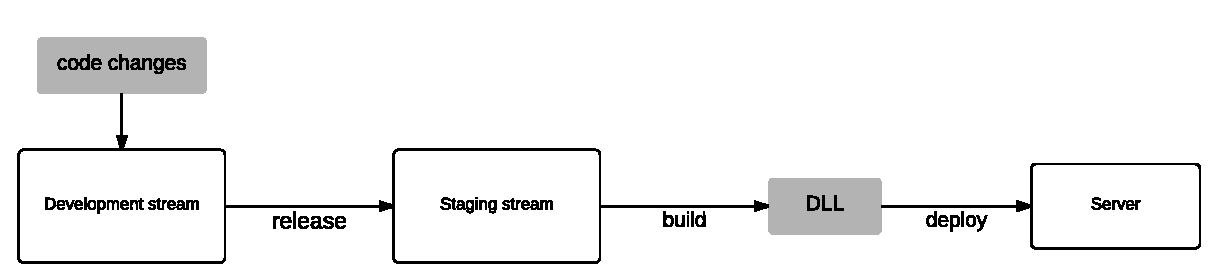
\includegraphics[width=13cm]{img/service-implementation.pdf}}
\caption{Process of deployment of implementation changes}
\label{fig:service-implementation}
\end{figure} 

\bigskip

On the server is just one version of the code. If another version is needed to be available it has to be deployed on another server. Then customers are using different servers, as shown on the image \ref{fig:consumer-server}

/TODO unfinished section

\begin{figure}[htp] \centering{
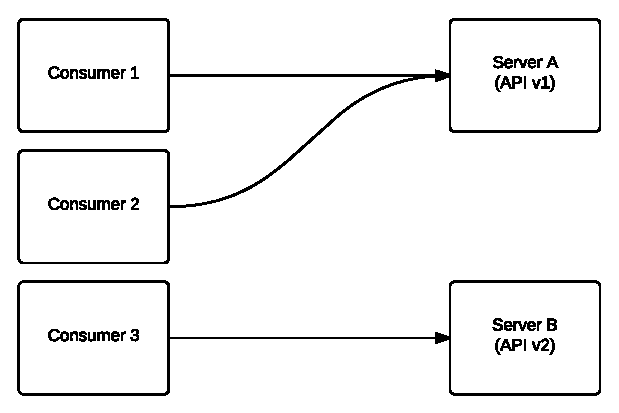
\includegraphics[width=10cm]{img/consumer-server.pdf}}
\caption{}
\label{fig:consumer-server}
\end{figure} 

\section{Service interface versioning}
\label{sec:interfaceversioning}

The service layer of an application which is developed by provider is composed of projects containing services. These services represent the service interface as the access point for consumer. Services contains methods (actions) which ensure operations over the services. The design is shown on Figure \ref{fig:service-layer-design}

\begin{figure}[htp] \centering{
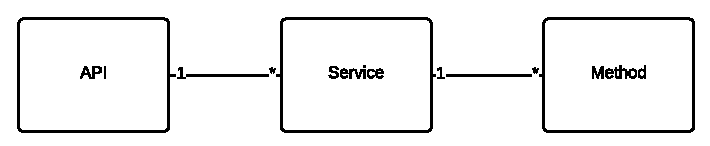
\includegraphics[width=11cm]{img/service-layer-design.pdf}}
\caption{Design of service layer}
\label{fig:service-layer-design}
\end{figure} 

This interpretation of service versioning is the most interesting for the analysis and brings various approaches. The versioning of services is quite young topic and there are still very vibrant discussions of the best approach. The analysis is executed in chapter \ref{chap:versionaccess}.

%Each version has its own implementation and is distinguishably addressed.

TODO unfinished

%Versioning management of services requires the proper definition of following concepts \cite{website:versioning-in-soa}:
%what will be versioned and how, the life-cycle of the versions and the access to the version.
%\begin{enumerate}
 % \item Units of versioning
 % \item Service changes, constituting a new version
 % \item Service version life-cycle considerations
 % \item Version deployment/access approaches
%\end{enumerate}

\section{Versioning strategy}
\label{sec:version-strategy}
There is a need to specify a set of rules to version services consistently. This rules form the versioning strategy. They are related to release of a new version of services or number of services which should be active at the same time. The rules are the matter of SOA governance. There isn't single correct way to govern the service versioning. Defined strategies should be followed and practiced during whole service lifecycle \cite{soa-governance}:

\begin{description}
  \item[Strict] 
  Any change of a service results in a new version. This strategy does not support backward or forward compatibility.
  \item[Flexible]
  Any incompatible changes result in a new version and the service design supports backward compatibility.
  \item[Loose]
  Any incompatible changes result in a new version and the service design supports backward and forward compatibility.
\end{description}

\subsection{Version identifiers}
Identification of the version is one of the fundamental design patterns. Version is indicated by decimals separated by periods. The version number length and common meaning of the digits should be established as a part of the versioning strategy. Every digit increments releatively to significance of the change. It is usually composed from two to four digits X.Y.Z.R.

Explanation of the digits \cite{soa-governance}:

\begin{enumerate}
  \item[Major changes X] \hfill \\
  Major changes are non-backward compatible changes, after a major change the new document schema is no longer compatible with the old one. These changes break the usage of the service by the consumer. They are imposed to the new version and consumers need to adjust their programs to switch to this version. Breaking changes can be performed by adding or removing an enumeration, removing or renaming a global type or element, changing the optionality of an element from optional to required.
  
    \item[Minor changes Y] \hfill \\
  Minor changes are backward-compatible changes. The changes do not impact consumers, the new version continue to support the consumers working with the old version. Examples can be new optional element to existing type, a change of optionality of a local element from required or optional, adding global type or global element, etc.
  
  \item[Patch version Z] \hfill \\  
  Patch version Z is incremented if only backwards compatible bug fixes are introduced. A bug fix is defined as an internal change that fixes incorrect behavior.
  
  \item[Revisions R] \hfill \\  
  Revisions are changes without semantic content, for example formatting, comments, etc. They do not affect the functionality of the service and service consumers.
\end{enumerate} 

Using version identifiers to express the compatibility by incrementing major and minor numbers serve to compatibility guarantee. There is another approach to indicate the version of services related to amount of work. The number increment according to effort which have been dedicated to the change. The big effort increments the major number and modest effort the minor number. This two approaches can be combined and in most cases they are, preserving mainly the compatibility guarantee and less often communicating the effort made. \cite{soa-governance}


\subsection{Service version life-cycle}
Service life-cycle defines the time period in which a version should be maintained. When the time is short, customers have not enough time for their upgrades required in order to switch on new verion. On the other hand when the period is too long, too many versions of service have to be maintained. The suitable time span is a result of consideration of individual organization with respect to their capability to deal with changes.

Product version should be always compatible with consumers usage. When a new version of the service method is released, it is needed to have the old one present in the implementation if any of the consumers operate with it. When the service method is going to be replaced by new one, it has to be held so that do not impact any consumer. It can be signed as deprecated, which do not influence its usage from the point of view of the consumer, but it means that provider waits that all consumers switch to the new implementation. When the deprecated method stops to be used, it can be safely removed. 

This lifecycle is possible only when the service method versioning approach is implemented, in case of whole-service versioning, when the service is given into state deprecated, it is equivalent to its remove, it is needed the new agreement between the provider and consumer so that consumer have to implement changes to use the new service %or just keep using the older version. 
The whole-service versioning provides less flexibility.

\section{Units of versioning}
It is needed to define what will be versioned. Most frequent are three possibilities, versioning of project, of services contained in project or of service methods. The relationship between this is shown in Figure \ref{fig:service-layer-design}.


\subsection{Versioning of project}
  /TODO 
\subsection{Versioning of service}
  The whole service is versioned with all its methods. This approach is working well with the object-oriented and the component-base development. It's not appropriate with coarse-grained services (\ref{sec:granularity}). \cite{website:versioning-in-soa} 
  
  This approach doesn't provide much flexibility.
  
\subsection{Versioning of service method}
  In most cases the change arises just in a method or some methods of the service. It is not necessary to version the whole service, but there is an option to version just these operations.
  The benefits of this approach are less code which is deployed because just a changed methods are redeployed in a new version. All services are immutable, their name and classification remain unchanged when there is a method added. The changes concern just a consumers which use the method, instead of consumers of the service containing changed method. 
  When the versioning of method is used it is needed to deploy each method with its own endpoint address, the advantage is that the \gls{sla} is provided for the method so that it is not changed the SLA of the same service.
  Moreover the addressing schema becomes more complex, the consumer has to specify not just the service but also the method and version of method which wants to use.
In spite of the more elaborate routing this possibility of versioning offers more flexibility. It adapts the services versioning to versioning practices of commonly used programming languages. 
Other benefit of this approach is deprecation, an old method which has new version can be signed as deprecated. The method can become deprecated when a better alternative is implemented but there are still consumers which use the old one. This method can remain in service until all consumers switch to the newest method.


%\subsection{Version definition}
%It is necessary to analyze the services/methods from the point of view of changes, their impact on the consumer. Analysis of possible changes deals with influence of change on the consumers execution and consequently defines the changes which will break it. When the change of the service or method is breaking it leads to the creation of new version.

%The components of the service are interface and message, both of them could be changed and cause the release of new version.

%\subsubsection{Interface changes}
A change of interface has significant impact on the consumer, it requires many modification of customers implementation or even completely new service. The deprecation of a method is equivalent to its removal and should occur rarely.
%When following semantic messages model, the interface is never changed. Advantage of this approach has source in the fact that all changes can be done just within the methods of service. 
When the methods are units of versioning they are deployed individually and new methods can be added without any impact on existing consumer. When the method is going to be removed, it is first deprecated, so that is still kept around the service and could be used until all consumers stop to use it. The changes are contained in messages and are not shown within the interface.
Than as seen it is better to design the versioning definition in order to not include the interface changes.



%\subsubsection{Message changes}
%When using the semantic message model the changes of service interface do not change the interface itself but are contained in message. The message is created by a schema which describes its content. Changes in schema can provide different cases of compatibility with actual implementation and can be divided in three categories:

%\subsection{Version access}
%It is needed to define how different consumers of services are accessing its version of the service. There are several approaches everyone has its pros and cons. The access possibilities are described in separate chapter \ref{chap:versionaccess}.

%\section{Versioning service implementation}
%Besides versioning the service interface, it is possible to consider an implementation. The underlying implementation can changed without affecting the interface itself. 
